\documentclass[../../main/main.tex]{subfiles}
\graphicspath{{./figures/}}

\dominitoc
\faketableofcontents

% \renewcommand{\mtcSfont}{\small\bfseries}
% \renewcommand{\mtcSSfont}{\footnotesize}
\mtcsettitle{minitoc}{}
\mtcsetrules{*}{off}

\makeatletter
\renewcommand{\@chapapp}{\'Electrocin\'etique -- chapitre}
\renewcommand{\chaplett}{E}
\makeatother

% \toggletrue{student}
% \toggletrue{corrige}
% \renewcommand{\mycol}{black}
% \renewcommand{\mycol}{gray}

\hfuzz=5.002pt

\begin{document}
\setcounter{chapter}{3}

\settype{book}
\settype{prof}
\settype{stud}

\chapter{Oscillateur harmonique}

\vspace*{\fill}

\begin{tcn}(appl)<ctc>"somm"'t'{Sommaire}
	\let\item\olditem
	\vspace{-15pt}
	\minitoc
	\vspace{-25pt}
\end{tcn}

\begin{tcn}[sidebyside](appl)<ctb>"how"'t'{Capacités exigibles}
	\begin{itemize}[label=\rcheck]
		\item Analyser, sur des relevés expérimentaux, l'évolution de la forme des
		      régimes transitoires en fonction des paramètres caractéristiques.
		\item Prévoir l'évolution du système à partir de considérations
		      énergétiques.
		\item Écrire sous forme canonique l'équation différentielle afin
		      d'identifier la pulsation propre et le facteur de qualité.
	\end{itemize}
	\tcblower
	\begin{itemize}[label=\rcheck]
		\item Établir et reconnaître l'équation différentielle qui caractérise un
		      oscillateur harmonique~; la résoudre compte tenu des conditions
		      initiales.
		\item Caractériser l'évolution en utilisant les notions d'amplitude, de
		      phase, de période, de fréquence, de pulsation.
		\item Réaliser un bilan énergétique.
	\end{itemize}
\end{tcn}

\vspace*{\fill}
\newpage
\vspace*{\fill}

%\vspace{-15pt}
\begin{tcn}[%
		sidebyside, fontupper=\small, fontlower=\small
	](appl)<ctb>"chek"'t'{L'essentiel}
	\begin{tcn}[nsp](defi)<ctc>'t'{Définitions}
		\tcblistof[\paragraph*]{defi}{\hspace*{4.8pt}}
	\end{tcn}
	% \begin{tcn}[nsp](rapp)<ctc>'t'{Rappels}
	% 	\tcblistof[\paragraph*]{rapp}{\hspace*{4.8pt}}
	% \end{tcn}
	\begin{tcn}[nsp](prop)<ctc>'t'{Propriétés}
		\tcblistof[\paragraph*]{prop}{\hspace*{4.8pt}}
		% \tcblistof[\paragraph*]{loi}{\hspace*{4.8pt}}
		% \tcblistof[\paragraph*]{theo}{\hspace*{4.8pt}}
	\end{tcn}
	% \begin{tcn}[nsp](loi)<ctc>'t'{Lois}
	% 	\tcblistof[\paragraph*]{loi}{\hspace*{4.8pt}}
	% \end{tcn}
	% \begin{tcn}[nsp](coro)<ctc>'t'{Corollaires}
	%   \tcblistof[\paragraph*]{coro}{\hspace*{4.8pt}}
	% \end{tcn}
	% \begin{tcn}[nsp](demo)<ctc>'t'{Démonstrations}
	% 	\tcblistof[\paragraph*]{demo}{\hspace*{4.8pt}}
	% 	\tcblistof[\paragraph*]{prev}{\hspace*{4.8pt}}
	% \end{tcn}
	% \begin{tcn}[nsp](inte)<ctc>'t'{Interprétations}
	% 	\tcblistof[\paragraph*]{inte}{\hspace*{4.8pt}}
	% \end{tcn}
	% \begin{tcn}[nsp](impl)<ctc>'t'{Implications}
	% 	\tcblistof[\paragraph*]{impl}{\hspace*{4.8pt}}
	% \end{tcn}
	% \begin{tcn}[nsp](tool)<ctc>'t'{Outils}
	% 	\tcblistof[\paragraph*]{tool}{\hspace*{4.8pt}}
	% \end{tcn}
	% \begin{tcn}[nsp](nota)<ctc>'t'{Notations}
	% 	\tcblistof[\paragraph*]{nota}{\hspace*{4.8pt}}
	% \end{tcn}
	% \begin{tcn}[nsp](appl)<ctc>'t'{Applications}
	% 	\tcblistof[\paragraph*]{appl}{\hspace*{4.8pt}}
	% \end{tcn}
	% \begin{tcn}[nsp](rema)<ctc>'t'{Remarques}
	%   \tcblistof[\paragraph*]{rema}{\hspace*{4.8pt}}
	% \end{tcn}
	% \begin{tcn}[nsp](exem)<ctc>'t'{Exemples}
	%   \tcblistof[\paragraph*]{exem}{\hspace*{4.8pt}}
	% \end{tcn}
	% \begin{tcn}[nsp](ror)<ctc>"hart"'t'{Points importants}
	%   \tcblistof[\paragraph*]{ror}{\hspace*{4.8pt}}
	% \end{tcn}
	% \begin{tcn}[nsp](impo)<ctc>'t'{Erreurs communes}
	%   \tcblistof[\paragraph*]{impo}{\hspace*{4.8pt}}
	% \end{tcn}
	\tcblower
	% \begin{tcn}[nsp](defi)<ctc>'t'{Définitions}
	%   \tcblistof[\paragraph*]{defi}{\hspace*{4.8pt}}
	% \end{tcn}
	% \begin{tcn}[nsp](rapp)<ctc>'t'{Rappels}
	%   \tcblistof[\paragraph*]{rapp}{\hspace*{4.8pt}}
	% \end{tcn}
	% \begin{tcn}[nsp](prop)<ctc>'t'{Propriétés}
	% \tcblistof[\paragraph*]{prop}{\hspace*{4.8pt}}
	% \tcblistof[\paragraph*]{loi}{\hspace*{4.8pt}}
	% \tcblistof[\paragraph*]{theo}{\hspace*{4.8pt}}
	% \end{tcn}
	% \begin{tcn}[nsp](coro)<ctc>'t'{Corollaires}
	%   \tcblistof[\paragraph*]{coro}{\hspace*{4.8pt}}
	% \end{tcn}
	\begin{tcn}[nsp](demo)<ctc>'t'{Démonstrations}
		\tcblistof[\paragraph*]{demo}{\hspace*{4.8pt}}
		% \tcblistof[\paragraph*]{prev}{\hspace*{4.8pt}}
	\end{tcn}
	\begin{tcn}[nsp](inte)<ctc>'t'{Interprétations}
		\tcblistof[\paragraph*]{inte}{\hspace*{4.8pt}}
	\end{tcn}
	% \begin{tcn}[nsp](impl)<ctc>'t'{Implications}
	% 	\tcblistof[\paragraph*]{impl}{\hspace*{4.8pt}}
	% \end{tcn}
	% \begin{tcn}[nsp](tool)<ctc>'t'{Outils}
	%   \tcblistof[\paragraph*]{tool}{\hspace*{4.8pt}}
	% \end{tcn}
	% \begin{tcn}[nsp](nota)<ctc>'t'{Notations}
	% 	\tcblistof[\paragraph*]{nota}{\hspace*{4.8pt}}
	% \end{tcn}
	% \begin{tcn}[nsp](odgr)<ctc>'t'{Ordres de grandeur}
	% 	\tcblistof[\paragraph*]{odgr}{\hspace*{4.8pt}}
	% \end{tcn}
	% \begin{tcn}[nsp](appl)<ctc>'t'{Applications}
	% 	\tcblistof[\paragraph*]{appl}{\hspace*{4.8pt}}
	% \end{tcn}
	% \begin{tcn}[nsp](rema)<ctc>'t'{Remarques}
	%   \tcblistof[\paragraph*]{rema}{\hspace*{4.8pt}}
	% \end{tcn}
	% \begin{tcn}[nsp](exem)<ctc>'t'{Exemples}
	% 	\tcblistof[\paragraph*]{exem}{\hspace*{4.8pt}}
	% \end{tcn}
	\begin{tcn}[nsp](ror)<ctc>"hart"'t'{Points importants}
		\tcblistof[\paragraph*]{ror}{\hspace*{4.8pt}}
	\end{tcn}
	\begin{tcn}[nsp](impo)<ctc>'t'{Erreurs communes}
		\tcblistof[\paragraph*]{impo}{\hspace*{4.8pt}}
	\end{tcn}
\end{tcn}

\vspace*{\fill}

Dans le chapitre précédent, nous avons vu des systèmes qui présentent un régime
transitoire caractérisé par des exponentielles croissantes ou décroissantes. En
combinant deux de ces composants, on trouve alors des régimes transitoires
caractérisé par une combinaison d'exponentielles, exprimée sous la forme de
fonctions sinusoïdales. Regardons un exemple.

\vspace*{\fill}

\newpage

\section{Introduction}

\subsection{Signal sinusoïdal}

\begin{tcb}[label=def:signsu, sidebyside, righthand ratio=.4]
	(defi){Signal sinusoïdal}
	Un signal sinusoïdal est un signal de la forme
	\psw{%
		\[
			\boxed{s(t) = A\cos(\wt + \f_0)}
		\]
	}%
	$A$ est l'\textit{amplitude}, telle que
	\psw{%
		\[
			A = \frac{s_{\max} - s_{\min}}{2}
		\]
	}%
	$\phi(t) = \wt +\f_0$ est la \textit{phase instantanée} du signal, avec
	\begin{center}
		\psw[limegreen]{%
			$\w$ la pulsation
		}%
		$\qqet$
		\psw[cornflowerblue]{%
			$\f_0$ la phase initiale
		}%
	\end{center}
	La pulsation représente la \textbf{vitesse de variation de la phase}.
	Pour un tour de $2\pi\,\si{rad}$, on a
	\psw{%
		\[
			\boxed{\w = \frac{2 \pi}{T} = 2\pi f}
			\Lra
			\boxed{T = \frac{2\pi}{\w}}
		\]
	}%
	% \vspace*{-20pt}
	% \begin{center}
	% 	\begin{tikzpicture}[]
	% 		\node[anchor=center] (name) at (0,0)
	% 		{\textcolor{cornflowerblue}{$\w$}$t$+\textcolor{limegreen}{$\f_0$}};
	% 		\node[inner sep=0] (datab) at ([shift={(0,3pt)}]name.south west) {};
	% 		\node[inner sep=0] (biasb) at ([shift={(0,3pt)}]name.south east) {};
	% 		\node[below left =.5cm and .5cm of datab, color=cornflowerblue] (data)
	% 		{pulsation};
	% 		\node[below right=.5cm and .5cm of biasb, color=limegreen] (bias)
	% 		{phase initiale};
	% 		\draw[-stealth] (data) -- (datab);
	% 		\draw[-stealth] (bias) -- (biasb);
	% 	\end{tikzpicture}
	% \end{center}
	\vspace{-15pt}
	\tcblower
	\begin{center}
		\sswitch{%
			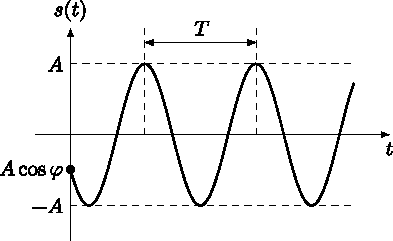
\includegraphics[width=\linewidth, draft=true]{onde_pres}
		}{%
			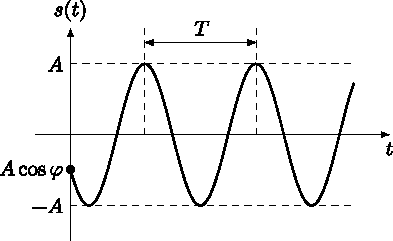
\includegraphics[width=\linewidth]{onde_pres}
		}%
		\captionof{figure}{}
	\end{center}
	\tcbsubtitle{\fatbox{Unités}}
	\psw{%
		La phase s'exprime en \textbf{radians}~; la pulsation en
		\textbf{$\si{rad.s^{-1}}$}.
	}%
	\vspace{-15pt}
\end{tcb}

\begin{tcb}[sidebyside, righthand ratio=.3]
  (inte)<lftt>"bulb"{Astuce de représentation}
	Par la nature de l'exponentielle, on peut plutôt représenter $s(t)$ à l'aide
	d'une exponentielle complexe~:
	\psw{%
		\[
			\boxed{\xul{s}(t) = A \exr^{\jj(\wt+\f_0)}}
		\]
	}%
	Pour retrouver la valeur réelle du signal, on en prend simplement la partie
	réelle.
	% Cette représentation a l'avantage de se représenter effectivement la
	% \textbf{phase} comme un \textbf{angle}, et donc la \textbf{pulsation} comme
	% la \textbf{vitesse de phase}.
	\tcblower
	\begin{center}
    \sswitch{%
          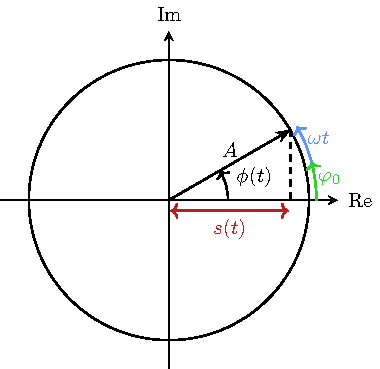
\includegraphics[width=\linewidth, draft=true]{onde_pres-xy}
    }{%
		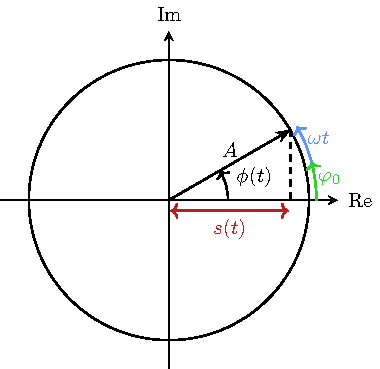
\includegraphics[width=\linewidth]{onde_pres-xy}
    }%
    \vspace{-15pt}
		\captionof{figure}{}
	\end{center}
\end{tcb}

\subsection{Équation différentielle oscillateur harmonique}

\begin{tcbraster}[raster columns=2, raster equal height=rows]
	\begin{tcb}[label=prop:eqdiffoh,
			list entry={\lte\theprop~:~Équation différentielle harmonique}]
		(prop){Équa$^\circ$ différentielle}
		Un oscillateur harmonique à un degré de liberté est un système dont
		l'évolution temporelle est décrite par une grandeur $x(t)$ solution
		d'une équation différentielle du type~:
		\psw{%
		\[
			\boxed{ \dv[2]{x}{t} + \w_0{}^2x = \w_0{}^2x_{\rm eq}}
		\]
		}%
		Avec $x_{\rm eq}$ la position d'équilibre du système et $\w_0$ la
		pulsation \textbf{propre}.
	\end{tcb}
	\begin{tcb}[label=prop:soluoh,
			list entry={\lte\theprop~:~Solutions harmoniques}]
		(prop)'r'{Solu$^\circ$ harmoniques}
		La forme générale des solutions d'un oscillateur harmonique s'écrit de
		manière équivalente
		\psw{%
			\begin{empheq}[box=\fbox]{gather*}
				x(t) = A'\cos(\w_0 t + \f_0) + x_{\rm eq}\\
				x(t) = A\cos(\w_0 t) + B\sin(\w_0 t) + x_{\rm eq}
			\end{empheq}
		}%
		avec $A'$, $\f_0$, $A$, $B$ des \textit{constantes d'intégration}.
	\end{tcb}
\end{tcbraster}

\subsection{Changement de variable~: de général à homogène}
Au cours du chapitre précédent, nous avons vu la méthode pour résoudre des
équations différentielles du premier ordre. Nous avons pu remarquer que les
équations différentielles entre les échelons montants et descendants étaient en
tout point similaire si ce n'est pour la présence ou non d'un second membre,
impliquant la recherche d'une solution particulière ou non.

Le changement de variable permet \textbf{d'éviter de
	chercher une solution particulière constante}.

\begin{tcb}[label=prop:chvar, sidebyside](prop){Changement de variable}
	Si $x(t)$ est solution de
	\psw{%
	\[
		\boxed{ \dv[2]{x}{t} + \w_0{}^2x = \w_0{}^2x_{\rm eq}}
	\]
	}%
	\tcblower
	alors $y(t) = x(t) - x_{\rm eq}$ est solution de
	\psw{%
		\[
			\boxed{ \dv[2]{y}{t} + \w_0{}^2y = 0}
		\]
	}%
\end{tcb}
\begin{tcb}(appl)<lftt>{Changement de variable}
	Résoudre l'équation du circuit RL montant par changement de variable.
	\tcblower
	\begin{isd}
		\psw{%
			L'équation différentielle totale s'écrit
			\[
				\boxed{
					\dv{i}{t} + \frac{1}{\tau}i(t) =
					\frac{1}{\tau}\frac{E}{R}
				}%
				\Lra
				\dv{i}{t} + \frac{i-\frac{E}{R}}{\tau} = 0
			\]
			On peut donc définir
			\[
				i_h(t) = i(t) - \frac{E}{R} \quad \Ra \quad \dv{i_h}{t} = \dv{i}{t} + 0
			\]
			donc $i_h$ est solution de
			\[
				\dv{i_h}{t} + \frac{i_h}{\tau} = 0
			\]
		}
		\vspace{-15pt}
		\tcblower
		\psw{%
			de solution générale
			\[
				i_h(t) = A\exr^{-t/\tau}
			\]
			On peut directement chercher l'expression de $A$ par CI~:
			\[
				i_h(0) = \underbracket[1pt]{i(0)}_{=0} - \frac{E}{R} = A
			\]
			Et en ré-isolant $i(t)$, on trouve bien
			\[
				\boxed{i(t) = \frac{E}{R}\left( 1 - \exr^{-t/\tau} \right)}
			\]
		}%
		\vspace{-15pt}
	\end{isd}
	\vspace*{-30pt}
\end{tcb}

\subsection{Exemple expérimental~: l'oscillateur LC}

Soit le circuit suivant sous un échelon de tension descendant. On observe la
tension $u_C(t)$ avec un oscilloscope dont la courbe est représentée à droite.
\textbf{Une simulation est disponible en
	ligne\ftn{\url{https://tinyurl.com/yl9rvpqg}}}.

\begin{minipage}{0.50\linewidth}
	\begin{center}
		\sswitch{%
			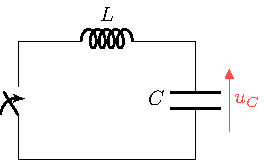
\includegraphics[width=.7\linewidth, draft=true]{lc_descendant}
		}{%
			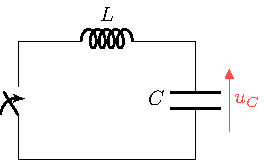
\includegraphics[width=.7\linewidth]{lc_descendant}
		}%
		\captionof{figure}{}
	\end{center}
\end{minipage}
\begin{minipage}{0.50\linewidth}
	\begin{center}
		\sswitch{%
			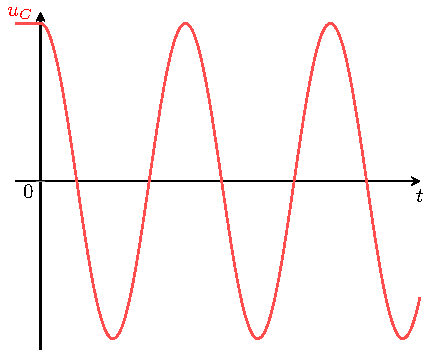
\includegraphics[width=.7\linewidth,
				draft=true]{carac-lc_descendant-harmonique-intro}
		}{%
			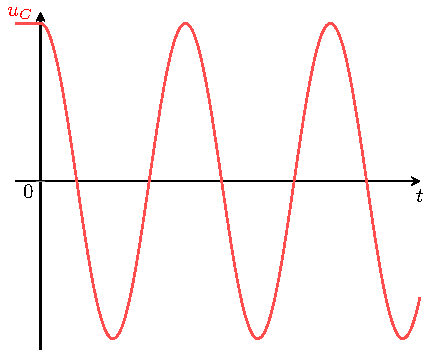
\includegraphics[width=.7\linewidth]{carac-lc_descendant-harmonique-intro}
		}%
		\captionof{figure}{}
	\end{center}
\end{minipage}
On remarque que la tension aux bornes du condensateur réalise des
d'oscillations sinusoïdales amorties. En fonction des valeurs des
caractéristiques des composants, on trouve~:
\begin{itemize}
	\item Pour $C_1 = \SI{80}{nF}$ et $L_1 = \SI{43}{mH}$, un période de $T_1 =
		      \SI{364}{\micro s}$~;
	\item Pour $C_2 = \SI{20}{nF}$ et $L_2 = \SI{43}{mH}$, un période de $T_2 =
		      \SI{184}{\micro s}$~;
\end{itemize}

\begin{tcn}(obsv)<lftt>{Analyse}
	Lorsque l'on excite le système LC, la tension aux bornes du condensateur
	\textbf{oscille} de façon \textbf{régulière et sinusoïdale}, avec une
	\textbf{fréquence} qui ne \textbf{dépend pas de l'amplitude} de l'excitation
	mais \textbf{dépend} des caractéristiques de l'oscillateur (\textbf{capacité}
	du condensateur et \textbf{inductance} de la bobine).
\end{tcn}

\section{Circuit LC régime libre}
\label{sec:lclibre}

\subsection{Présentation}

\begin{tcb*}[sidebyside, righthand ratio=.30](defi){Circuit LC libre}
	\begin{itemize}
		\item Il est constitué de l'association en série d'une bobine et d'un
		      condensateur idéaux.
		\item \textbf{On suppose le condensateur initialement chargé}
		      % ~:
		      %   \fbox{$u_C(0^-) = E$ \underline{et} $i(0^-) = 0$}
		      %   \smallbreak
		      %   (condensateur chargé $\equiv$ interrupteur ouvert).
		\item À $t=0$, on coupe le générateur.
	\end{itemize}
	\tcblower
	\begin{center}
		\sswitch{%
			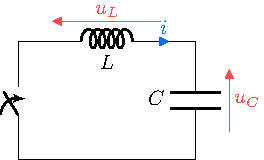
\includegraphics[width=\linewidth, draft=true]{lc_descendant-intens}
		}{%
			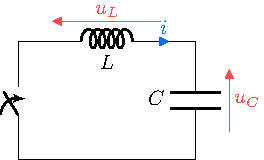
\includegraphics[width=\linewidth]{lc_descendant-intens}
		}%
		\captionof{figure}{}
	\end{center}
\end{tcb*}

\subsection{Équation différentielle du circuit}
\begin{tcb*}[label=demo:eqdiffrc](demo){Équation diff. LC libre}
	Avec la loi des mailles,
	\psw{%
		\begin{DispWithArrows*}[]
			u_L + u_C &= 0
			\Arrow{$\DS u_L = L \dv{i}{t}$\\ et $\DS i = C \dv{u_C}{t}$}
			\\\Lra
			LC \dv[2]{u_C}{t} + u_C          &= 0
			\Arrow{forme canonique}
			\\
			\Lra \dv[2]{u_C}{t} + \frac{1}{LC}u_C &= 0
		\end{DispWithArrows*}
		D'où le résultat. $L$ assure $i(0^+) = 0$ et $C$ assure $u_C(0^+) = E$
		par continuité.
	}%
\end{tcb*}
\begin{tcb*}[label=prop:eqdiffrc, sidebyside, righthand ratio=.4](prop){Équation diff. LC libre}
	L'équation différentielle de la tension $u_C(t)$ aux bornes d'un
	condensateur dans un circuit LC en régime libre est
	\[
		\psw{%
			\boxed{\dv[2]{u_C}{t} + \w_0{}^2u_C = 0}
		}%
		\qav
		\psw{%
			\boxed{\w_0 = \frac{1}{\sqrt{LC}}}
		}%
	\]
	\tcblower
	Les conditions initiales (continuité de $u_C$ aux bornes de $C$
	et de $i$ traversant $L$) sont
	\psw{%
		\begin{empheq}[box=\fbox]{align*}
      u_C(0^-) &= u_C(0^+) = E\\
      i(0^-) &= i(0^+) = 0
		\end{empheq}
	}%
\end{tcb*}

\begin{tcb}[label=rema:unité](appl)<lftt>{Unité de $\w_0$}
	On peut vérifier à cette étape que $\w_0$ est bien homogène à l'inverse d'un
	temps. Pour ça, deux manières~:

	\begin{isd}[sidebyside align=top]
		\tcbsubtitle{\fatbox{Analyse directe}}
		Sachant que $RC$ et $L/R$ sont des temps (cf.\ chapitre précédent)~:
		\psw{%
			\begin{align*}
				\w_0{}^2 = \frac{1}{LC} =
				\frac{R}{LRC} =
				\underbrace{\left[ \frac{L}{R}
						\right]^{-1}}_{\si{s^{-1}}}\times
				\underbrace{\left[ RC \right]^{-1}}_{\si{s^{-1}}}
			\end{align*}
			Et on a bien $\w_0{}^2$ en \si{s^{-2}}, et donc $\w_0$ en \si{s^{-1}},
			les radians n'ayant pas de dimension.
		}%
		\tcblower
		\tcbsubtitle{\fatbox{Analyse indirecte}}
		En effet, l'équation différentielle est forcément une équation homogène.
		Ainsi
		\psw{%
			\begin{equation*}
				\left[ \dv[2]{u_C}{t} \right] =
				\frac{\left[u_C\right]}{\left[\dt\right]^2}\\
				= \frac{\si{V}}{\si{s^2}}
			\end{equation*}
			et l'autre terme doit avoir la même unité~:
			\begin{equation*}
				\left[ \w_0{}^2u_C \right] = \left[ \w_0 \right]^2\times \left[
					u_C \right]\\
				= \si{V.s^{-2}}
			\end{equation*}
			On en déduit que $\w_0{}^2$ est de dimension \si{s^{-2}}, d'où la
			dimension de $\w_0$.
		}%
	\end{isd}
\end{tcb}

\subsection{Résolution de l'équation différentielle et graphique}
\begin{tcb*}[label=demo:rcsolu](demo){Solutions LC série descendant}
	L'équation étant déjà homogène, on injecte la forme générique~:
	\psw{%
		\[
			u_C(t) = K \exr^{rt}
			\Ra
			r^2 \times \cancel{K \exr^{rt}} + \w_0{}^2\cancel{K\exr^{rt}} = 0
			\Lra
			r_{\pm} = \pm \jw_0
		\]
	}%
	On écrit alors la forme réelle générale~:
	\psw{%
		\[
			u_C(t) = A\cos(\w_0 t) + B\sin(\w_0 t)
		\]
	}%
	\vspace{-15pt}
	\begin{isd}[interior hidden, sidebyside align=top]
		On trouve $A$ avec une condition initiale~:
		\psw{%
			\[
				u_C(0) = A\cos(0) + B\sin(0) = A
				\\\Lra
				\boxed{A = E}
			\]
		}%
		\tcblower
		On trouve $B$ avec l'autre condition initiale~:
		\psw{%
			\begin{gather*}
				\qty(\dv{u_C}{t})_0 =
				-A\w_0\sin(0) + B\w_0\cos(0) =
				B\w_0
				\\\text{or,} \quad
				i(0) = 0 = C \qty(\dv{u_C}{t})_0 = CB\w_0
				\Ra \boxed{B = 0}
			\end{gather*}
		}%
		\vspace{-15pt}
	\end{isd}
	\smallbreak
	On obtient ensuite $i$ avec la relation courant-tension~:
	\psw{%
		\[
			i(t) = C \dv{u_C}{t} = -CE \w_0 \sin(\w_0t)
		\]
	}%
	\vspace{-15pt}
\end{tcb*}

\begin{tcb*}(impo){Évaluation en 0 d'une dérivée}
	Il est malheureusement plus que commun de confondre la dérivée évaluée en 0,
	et la dérivée de la fonction évaluée en 0~:
	\psw{%
		\[
			\boxed{\qty(\dv{f}{t})_0 \neq \dv{f(0)}{t}}
		\]
	}%
	\textbf{Ça n'est pas parce qu'une fonction est nulle en un point que sa
		dérivée en ce point est nulle~!}
\end{tcb*}

\begin{tcb*}[label=prop:ucsolu, sidebyside, righthand ratio=.3]
	(prop){Solution LC descendant}
	La solution de l'équation différentielle de la tension $u_C(t)$
	d'un circuit LC en décharge avec $u_C(0) = E$ et $i(0) = 0$ donne~:
	\psw{%
		\begin{empheq}[box=\fbox]{align*}
      u_C(t) & = E\cos(\w_0t)
      \\
      i(t)   & = -CE\w_0\sin(\w_0t)
		\end{empheq}
	}%
	\tcblower
	\begin{center}
		\sswitch{%
			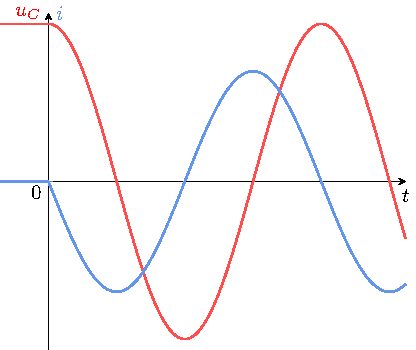
\includegraphics[width=\linewidth,
				draft=true]{carac-lc_descendant-harmonique}
		}{%
			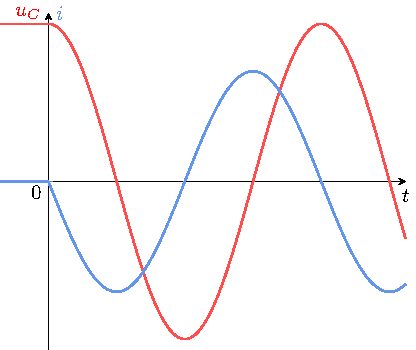
\includegraphics[width=\linewidth]{carac-lc_descendant-harmonique}
		}%
		\captionof{figure}{}
	\end{center}
\end{tcb*}

\begin{tcb}(inte)<lftt>"bulb"{Espace des phases LC}
  Il est utile d'observer la physique des systèmes oscillants non pas dans un
  espace (grandeur, temps) mais dans un espace \textbf{(grandeur,
    dérivée)}, qui permet plus rapidement de sonder son évolution~: c'est ce
  qu'on appelle \textbf{l'espace des phases}.
  \bigbreak
  Ici, la tension s'exprime comme un cosinus et l'intensité comme un sinus. Or,
  $-\sin(x) = \cos(x+\pi/2)$~: on dit qu'ils sont \textbf{déphasés de $\pi/2$}.
  Ils dessinent alors une \textbf{ellipse} dans l'espace des phases.
  \tcblower
  \begin{isd}[righthand ratio=.3]
      Le condensateur étant initialement chargé, l'intensité est nulle. Étant donné
    notre convention récepteur, lors de sa décharge l'intensité sera d'abord
    négative, et diminue jusqu'à s'annuler.
    \bigbreak
    Pendant cette décharge, la bobine a stocké de l'énergie, qu'elle ré-émet alors
    dans le circuit et recharge le condensateur~; l'intensité est alors positive.
    \bigbreak
    %
    % Par
    % exemple, le ressort lâché à $x_0$ et $v_0=0$ voit sa position diminuer
    % et sa vitesse augmenter (algébriquement) jusqu'à ce qu'il passe par sa
    % position d'équilibre ($x=0$) avec une vitesse extrémale $v_{\min}$,
    % avant de se comprimer en perdant de sa vitesse.
    % \bigbreak
    Comme il n'y a \textbf{pas de perte dans cette étape}, elle se répète
    \textbf{symétriquement} en revenant à son point de départ.
    \tcblower
    \begin{center}
      \sswitch{%
        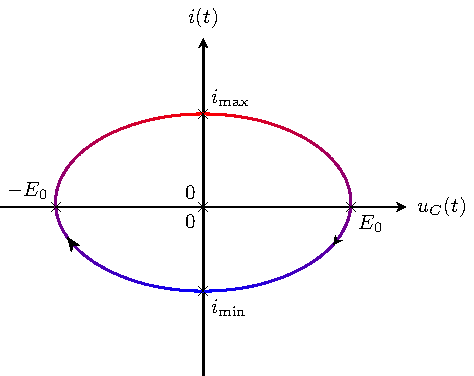
\includegraphics[width=\linewidth, draft=true]{carac-lc_descendant-xy}
      }{%
        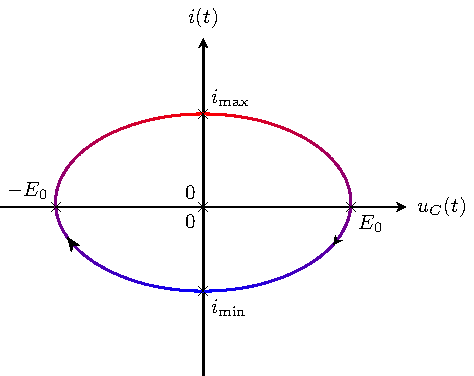
\includegraphics[width=\linewidth]{carac-lc_descendant-xy}
      }%
      \captionof{figure}{}
    \end{center}
  \end{isd}
\end{tcb}
\subsection{Bilan énergétique}
\begin{tcb*}[label=demo:rcenerg-charge](demo){Bilan d'énergie LC descendant}
  On fait un bilan de puissances avec la loi des mailles multipliée par $i$~:
  \psw{%
    \begin{DispWithArrows*}
      u_Ci + u_Li &= 0
      \Arrow{$i = C \dv{u_C}{t}$\\et $u_L = L \dv{i}{t}$}
      \\
      \Lra
      u_C\times C \dv{u_C}{t} + L \dv{i}{t}\times i &= 0
      \Arrow{$f \times f' = \left( \frac{1}{2}f^{2} \right)'$}
      \\\Lra
      \dv{}{t} \left( \frac{1}{2}Cu_C{}^2 + \frac{1}{2}Li^2 \right) &= 0
    \end{DispWithArrows*}
    On identifie l'intérieur de la parenthèse à l'énergie du système (car
    par définition $\Pc = \dv{\Ec}{t}$) pour avoir la propriété.
  }%
\end{tcb*}

\begin{tcb*}[label=prop:lcenerg-décharge, sidebyside, righthand ratio=.3]
  (prop){Bilan d'énergie LC descendant}
  L'énergie emmagasinée dans le circuit est
  \psw{%
	\[
		\boxed{\Ec = \frac{1}{2}Cu_C{}^2 + \frac{1}{2}Li^2}
	\]
  }%
  Elle est \textbf{conservée à chaque instant} et résulte de l'\textbf{échange
    périodique} d'énergie entre le condensateur et la bobine.
  \tcblower
  \begin{center}
    \sswitch{%
      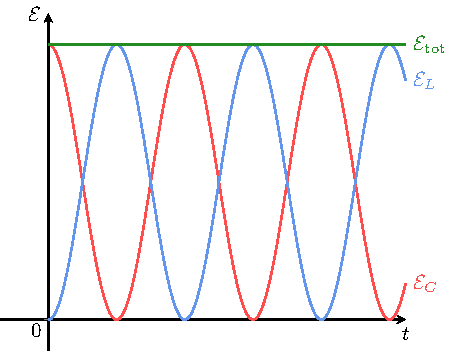
\includegraphics[width=\linewidth, draft=true]{carac-lc_descendant-bilan}
    }{%
      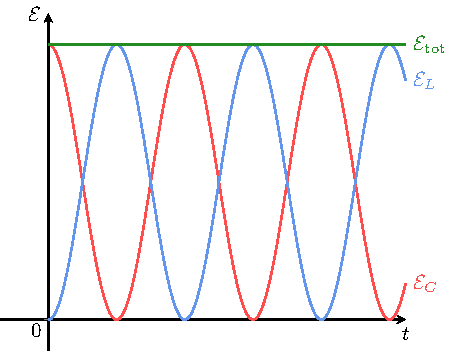
\includegraphics[width=\linewidth]{carac-lc_descendant-bilan}
    }%
    \captionof{figure}{}
  \end{center}
\end{tcb*}

\begin{tcb}[label=impl](rema)<lftt>{Vérification conservation de l'énergie LC}
	On vérifie avec les expressions analytiques trouvées, sachant que
	$\w_0{}^2 = (LC)^{-1}$~:
	\psw{%
		\begin{align*}
			\frac{1}{2}Cu_C(t)^2 & = \frac{1}{2}CE^2\cos^2(\w_0t)
			\\
			\text{et} \quad
			\frac{1}{2}Li(t)^2   & =
			\frac{1}{2}\underbracket[1pt]{LC^{2}\w_0{}^2}_{=C}E^2\sin^2(\w_0t)
			\\\Ra
			\Ec                  & =
			\frac{1}{2}CE^2 \left( \cos^2(\w_0t) + \sin^2(\w_0t) \right)
			= \frac{1}{2}CE^2 = \cte
			% \\\Lra
			% \Aboxed{\Ec          & = \frac{1}{2}CE^2 = \text{cste}}
		\end{align*}
		% Soit
		% \begin{equation*}
		% 	\boxed{\Ec = \frac{1}{2}CE^2 = \text{cste}}
		% \end{equation*}
	}%
  \vspace{-20pt}
\end{tcb}
\begin{tcb}[label=ror:amortissement](ror)<lftt>{Conclusion LC descendant}
	On retrouve bien des oscillations de la tension aux bornes de $u_C$ comme dans
	l'approche expérimentale, avec une période $T_0 = \frac{2\pi}{\w_0} =
		2\pi\sqrt{LC}$ qui augmente avec $L$ et $C$.
	\bigbreak
	Il n'y a donc \textbf{pas d'amortissement ici}~! En effet les composants
	utilisés ici sont idéaux, et conservent totalement l'énergie, il n'y a pas de
	raison d'en perdre.
	\bigbreak
	Il y a eu une simplification que l'on effectue souvent~:
	\textbf{on a négligé les effets dissipatifs}.
\end{tcb}

\section{Exemple harmonique mécanique~: ressort horizontal libre}

\subsection{Introduction}
% Soit le système masse-ressort horizontal représenté ci-après. Le ressort se
% déforme sous l'effet d'une contrainte en stockant l'énergie donnée, qu'il
% libère en reprenant sa forme quand la contrainte s'arrête.
\begin{tcb*}[label=defi:ressortdef, sidebyside, righthand ratio=.35,
  list entry={\lte\thedefi~:~Force de \textsc{Hooke}}]
	(defi){Force de \textsc{Hooke} de rappel d'un ressort}
	On définit la force de \textsc{Hooke} par~:
	\psw{%
		\begin{equation*}
			\boxed{\vv*{F}{\rm rappel} = \pm k(\ell(t) - \ell_0)\ux}
		\end{equation*}
	}%
	\vspace{-15pt}
	\begin{itemize}
		\item 
      \psw{%
        $k > 0$ la \textbf{constante de raideur} en \textbf{\si{N.m^{-1}}}~;
      }%
		\item 
      \psw{%
        $\ell_0$ sa \textbf{longueur à vide}~;
      }%
		\item 
      \psw{%
        $\ux$ un vecteur unitaire ($\norm{\ux} = 1$) dirigé selon $x$.
      }%
	\end{itemize}
  Le signe dépend de l'orientation du vecteur de base.
	% \tcbsubtitle{\fatbox{Unité}}
	% \psw{%
	% $k$ en $\si{N.m^{-1}}$ ($[\vv{F}] = [k][\ell]$)
	% }%
	\tcblower
	\begin{center}
    \sswitch{%
      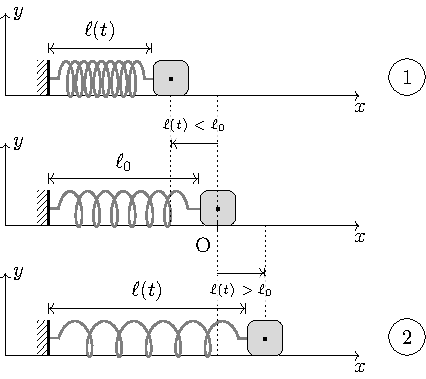
\includegraphics[width=\linewidth]{ressort_def-stud}
    }{%
      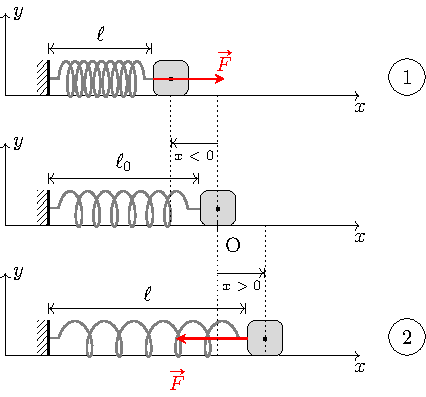
\includegraphics[width=\linewidth]{ressort_def}
    }%
		\vspace{-20pt}
    \captionsetup{justification=centering}
		\captionof{figure}
    {\\$\protect\Ff = \fbox{\psw{-}}k (\ell(t) - \ell_0) \protect\ux$}
	\end{center}
	% Si $\ell > \ell_0$, on a bien une force dirigée selon $-\ux$, (situation
	% \circled{2}), sinon dirigée selon $+\ux$.
\end{tcb*}

\subsection{Présentation}
\begin{tcb*}[label=def:ressortlibre, sidebyside](defi){Situation
			initiale et bilan des forces}
	\begin{itemize}[label=$\diamond$, leftmargin=10pt]
		\item[b]{Système}: 
      \psw{%
        \{point M\} de masse $m$
      }%
		\item[b]{Référentiel}: 
      \psw{%
        $\Rc\ind{sol}$ supposé galiléen
      }%
		\item[b]{Repère}: 
      \psw{%
        $(\Or', \ux, \uy)$ (voir schéma)
      }%
		\item[b]{Repérage}:
		      % \vspace{-15pt}
		      % \begin{center}
		      %  \hspace*{-10pt}
		      %  \fbox{Soit $x (t) = \ell(t) - \ell_0$ la position de la masse}
		      % \end{center}
      \psw{%
                  \[
                  \hspace{-15pt}
                  \vv{\rm OM} = (\ell(t)-\ell_0)\ux~;
                  \vf = \lp(t)\ux~;
                  \af = \lpp(t)\ux
                \]
      }%
      \vspace{-15pt}
		\item[b]{Position initiale}: 
      \psw{%
        ${\rm OM}(0) = L_0 > 0$
      }%
		\item[b]{Vitesse initiale}: 
      \psw{%
        $\vf(0) = \of$
      }%
	\end{itemize}
	\tcblower
	\begin{center}
		\sswitch{%
			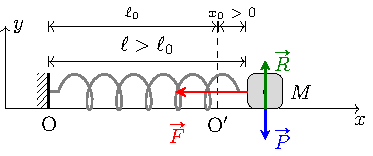
\includegraphics[width=\linewidth, draft=true]{ressort_libre}
		}{%
			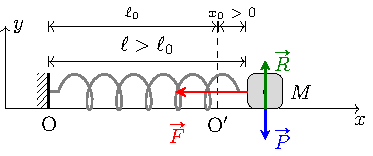
\includegraphics[width=\linewidth]{ressort_libre}
		}%
		\vspace{-20pt}
		\captionof{figure}{}
	\end{center}
	\begin{itemize}[label=$\diamond$, leftmargin=10pt]
		\item[b]{Bilan des forces~:}
		      \psw{%
			      \[
				      \begin{array}{ll}
					      \textbf{Poids}            & \Pf = m\gf = -mg \uy \\
					      \textbf{Réaction support} & \Rf = R\uy           \\
					      \textbf{Force de rappel}  & \Ff = -k (\ell(t) - \ell_0)\ux
				      \end{array}
			      \]
		      }%
	\end{itemize}
\end{tcb*}

\subsection{Équation différentielle et solution}

\begin{tcb*}[label=demo:solreslibre, sidebyside, sidebyside align=top]
  (demo){Équation et solution ressort libre}
  \tcbsubtitle{\fatbox{Équation}}
  La deuxième loi de \textsc{Newton}, ou \textbf{principe fondamental de la
    dynamique} (PFD) donne~:
  \psw{%
    \begin{gather*}
      \dv{\pf}{t} = m\af = \Pf + \vv{R} + \Ff\\
      \Lra m
      \mqty(
      \dv[2]{\ell}{t} \\
      0) = \mqty( -k (\ell(t) - \ell_0) \\
      -mg + R)
    \end{gather*}
  }%
  Sur l'axe $\ux$
  % \ftn{La projection sur $\uy$ montre que la réaction du support
  %   compense le poids.}
    on trouve alors
  \psw{%
		\[
			m \dv[2]{\ell}{t} + k \ell(t) = k \ell_0
      \Lra
      \boxed{\dv[2]{x}{t} + \w_0{}^{2}x = 0}
		\]
  }%
  \begin{gather*}
    \beforetext{avec}
    \psw{%
      x(t) = \ell(t) - \ell_0
    }%
    \\
    \beforetext{et}
      \psw{%
          \w_0{}^{2} = \frac{k}{m} \Ra \boxed{\w_0 = \sqrt{\frac{k}{m}}}
      }%
  \end{gather*}
  \tcblower
  \tcbsubtitle{\fatbox{Solution}}
  On écrit la forme générale~:
  \psw{%
		\[
			x(t) = A\cos(\w_0 t) + B\sin(\w_0 t)
		\]
  }%
  \vspace{-20pt}
  \begin{itemize}
    \item On trouve $A$~:
          \psw{%
			      \[
				      x(0) = \boxed{A = L_0 - \ell_0} = x_0
			      \]
          }%
          \vspace{-15pt}
    \item On trouve $B$~:
          \psw{%
            \begin{gather*}
              v(0) = 0 = \qty(\dv{x}{t})_0 = B\w_0
              \quad \Ra \boxed{B = 0}
            \end{gather*}
          }%
          \vspace{-15pt}
  \end{itemize}
  Donc
  \psw{%
		\[
			\boxed{x (t) = x_0\cos(\w_0t)}
		\]
  }%
  Or,
  \psw{%
    \[
      \boxed{v(t) = \dv{x}{t}}
    \]
  }%
  % On obtient ensuite $v$ avec la relation vitesse-position.
\end{tcb*}
\begin{tcb*}[label=prop:eqdiffreslibre, sidebyside, righthand ratio=.4]
  (prop){Équation et solution ressort libre}
  La position $x$ de la masse et la longueur $\ell$ du ressort sont régies par~:
    \begin{gather*}
      \psw{%
              \boxed{%
              \dv[2]{x}{t} + \w_0{}^2x = 0
              \Lra
              \dv[2]{\ell}{t} + \w_0{}^2\ell = \w_0{}^2\ell_0
            }
      }%
      \\\beforetext{avec la pulsation propre}
      \hspace{40pt}
      \psw{%
              \w_0 = \sqrt{\frac{k}{m}}
      }%
    \end{gather*}
  $\ell_0$ est donc la \textbf{longueur d'équilibre} du système.
  \tcblower
  La position $x$ et la vitesse $v$ ont pour expressions
  \psw{%
    \begin{empheq}[box=\fbox]{align*}
      x(t) &= x_0\cos(\w_0t)\\
      \text{et} \quad
      v(t) &= -x_0\w_0\sin(\w_0t)
    \end{empheq}
  }%
  avec $x_0 = L_0-\ell_0$ le déplacement initial.
\end{tcb*}

\begin{tcb*}[label=ror:ressortlibre, breakable](ror)<lftt>{Analogie LC-ressort}
  % Alors qu'on partait d'un système \textit{a priori} totalement différent, on
  % remarque que
  La physique des deux systèmes sont rigoureusement équivalentes
  puisque \textbf{régies par la même équation différentielle}.
  \bigbreak
  \noindent
  \begin{minipage}[c]{.70\linewidth}
    Il y a oscillation du ressort autour d'une position d'équilibre, ici
    $x\ind{eq}=0 \Lra \ell\ind{eq} = \ell_0$, comme $u_C$ oscille autour de
    0.
    \smallbreak
    On associe donc \fbox{$q$ à $x$} et \fbox{$i$ à $v$}, étant donné que pour
    un condensateur $i = \dv{q}{t}$ et que $v = \dv{x}{t}$.
    \smallbreak
    De plus c'est la \textbf{masse} qui impose l'inertie du mouvement, comme
    l'\textbf{inductance} est l'inertie de l'intensité.
    \smallbreak
    Finalement, $\w_0 = 1/\sqrt{LC}$ en électrocinétique et $\w_0 =
      \sqrt{k/m}$ en mécanique, donc on associe $k$ à $C^{-1}$.
  \end{minipage}
  \hfill
  \begin{minipage}[c]{.25\linewidth}
    % \captionof{table}{Correspondances}
    \centering
    \begin{tabular}{c@{$\longleftrightarrow$}c}
      \toprule Méca & Élec \\
      \midrule
      \psw{$x$} & \psw{$q$}
      \\
      \psw{$v$} & \psw{$i$}
      \\
      \psw{$m$} & \psw{$L$}
      \\
      \psw{$k$} & \psw{$C^{-1}$}
      \\
      \psw{$\sqrt{\frac{k}{m}}$} & \psw{$\frac{1}{\sqrt{LC}}$}
      \\
      \bottomrule
    \end{tabular}
  \end{minipage}
\end{tcb*}

\subsection{Bilan énergétique}

\begin{tcb*}[label=def:emeca, sidebyside,
  list entry={\lte\thedefi~:~Énergies d'un ressort}]
  (defi){Énergies potentielle élastique et mécanique}
	Le ressort emmagasine une énergie \textit{potentielle} lors de sa
	déformation, telle que
	\psw{%
		\[
			\boxed{
				\Ec_{p\rm, el} = \frac{1}{2}k(\ell-\ell_0)^2 = \frac{1}{2}kx^2
			}%
		\]
	}%
	\tcblower
	On définit alors l'énergie mécanique totale $\Ec_m$ du système par
		\[
	\psw{%
			\boxed{\Ec_m = \Ec_c + \Ec_{p\rm, el}}
	}%
  \qav
  \psw{%
    \Ec_c = \frac{1}{2}mv^2
  }%
		\]
	% avec, évidemment, $\Ec_c = \frac{1}{2}mv^2$.
\end{tcb*}

\begin{tcb}[fontupper=\Large, bld, cnt](ror){Bilan de puissance en méca}
	On effectue un bilan de puissance en écrivant le PFD multiplié par $v$~:
	$\Pc(\vv{F}) = \vv{F}\cdot \vv{v}$.
\end{tcb}

\begin{tcb*}[label=demo:emecacons](demo){Conservation énergie ressort}
	À partir du PFD~:
	\vspace{-15pt}
	\psw{%
		\begin{DispWithArrows*}[]
			m \dv[2]{x}{t} + kx &= 0
			\CArrow{$\times v$}
			\\\Lra
			m \dv[2]{x}{t} \dv{x}{t} + kx \dv{x}{t} &= 0
			\Arrow{$f \times f' = \left(\frac{1}{2}f^2\right)'$}
			\\\Lra
			\dv{}{t}
			\Big(
			\underbracket{\frac{1}{2}m \left( \dv{x}{t} \right)^2}_{\Ec_c} +
			\underbracket{\frac{1}{2}kx^2}_{\Ec_{p, \rm el}}
			\Big) &= 0
		\end{DispWithArrows*}
	}%
	\vspace{-15pt}
\end{tcb*}

	\begin{tcb*}[label=prop:emecacons, sidebyside, righthand ratio=.3]
    (prop){Conservation énergie ressort}
		Dans le système masse-ressort horizontal sans frottements, l'énergie
		mécanique est conservée~:
		\psw{%
			\[
				\boxed{\Ec_m = \cte}
				\Lra
				\boxed{\dv{\Ec_m}{t} = 0}
			\]
		}%
		\vspace{-15pt}
    \tcblower
		\begin{center}
			\sswitch{%
				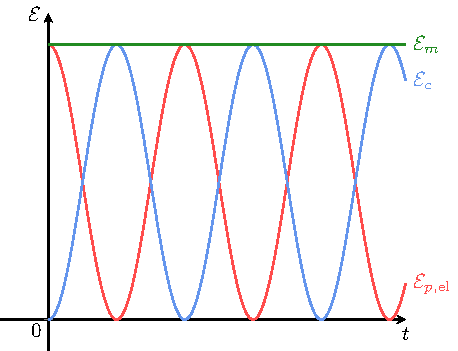
\includegraphics[width=\linewidth,
					draft=true]{carac-ressort_libre-bilan}
			}{%
				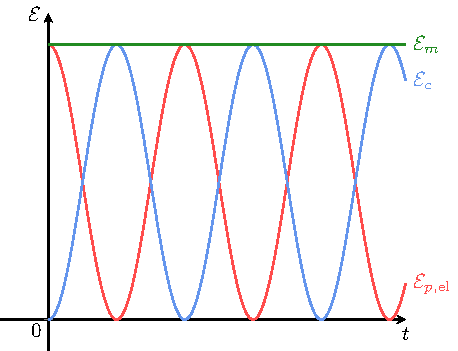
\includegraphics[width=\linewidth]{carac-ressort_libre-bilan}
			}%
			\captionof{figure}{}
		\end{center}
	\end{tcb*}
\begin{tcb}[label=rema](rema)<lftt>{Vérification conservation énergie ressort}
	On vérifie avec les expressions analytiques, sachant que
	$\w_0{}^2 = \frac{k}{m}$~:
	\psw{%
		\begin{align*}
			\frac{1}{2}kx^2 & = \frac{1}{2}kx_0{}^2\cos^2(\w_0t)
			\\
			\text{et} \quad
			\frac{1}{2}mv^2 & =
			\frac{1}{2}\underbracket[1pt]{m\w_0{}^2}_{=k}x_0{}^2\sin^2(\w_0t)
			\\\Ra
			\Ec_m           & =
      \frac{1}{2}kx_0{}^2 \left( \cos^2(\w_0t) + \sin^2(\w_0t) \right) =
      \frac{1}{2}kx_0{}^2 = \cte
		\end{align*}
		% Soit
		% \begin{equation*}
		% 	\boxed{\Ec_m = \frac{1}{2}kx_0{}^2 = \text{cste}}
		% \end{equation*}
	}%
\end{tcb}

\subsection{Analyse correspondance}
\begin{tcb}[width=\linewidth, sidebyside, righthand ratio=.3]
  (inte)<lftt>"bulb"{Espace des phases ressort libre}
	Le ressort lâché à $x_0$ et $v_0=0$ voit sa position diminuer
	et sa vitesse augmenter (algébriquement) jusqu'à ce qu'il passe par sa
	position d'équilibre ($x=0$) avec une vitesse extrémale $v_{\min}$,
	avant de se comprimer en perdant de sa vitesse.
	\bigbreak
	Comme il n'y a
	\textbf{pas de perte dans cette étape}, elle se répète
	\textbf{symétriquement} en revenant à son point de départ.
	\tcblower
	\begin{center}
		\sswitch{%
			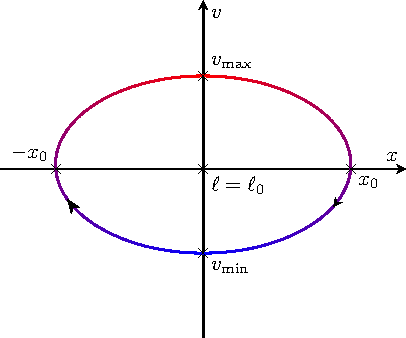
\includegraphics[width=\linewidth, draft=true]{carac-ressort_libre-xy}
		}{%
			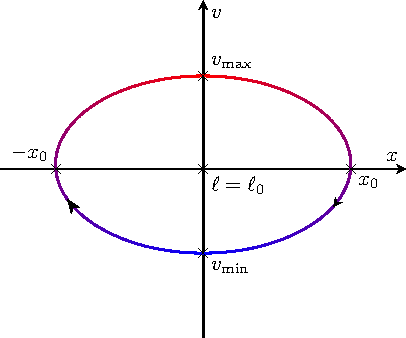
\includegraphics[width=\linewidth]{carac-ressort_libre-xy}
		}%
		\captionof{figure}{}
	\end{center}
\end{tcb}

\begin{tcb}[label=ror:harmotoamorti](ror)<lftt>{Conclusion harmonique}
	En réalité, les \textbf{frottements en mécanique existent}, et à chaque étape
	le système masse-ressort perd de l'énergie dans la dissipation par frottement
	créant de la chaleur. On va donc avoir une \textbf{trajectoire amortie} plus
	ou moins fortement.
	\bigbreak
	Dans le cas électrique, c'est la \textbf{résistance que nous avions négligée}
	alors qu'elle existe toujours~: notamment la bobine réelle est composée d'une
	bobine idéale et d'une résistance en série. C'est la résistance qui va
	\textbf{dissiper l'énergie} de l'oscillateur harmonique LC sous forme de
	chaleur par effet \textsc{Joule} et amortir l'oscillation de $u_C$.
\end{tcb}

\section{Complément~: circuit LC montant}

\subsection{Présentation}

\begin{tcb*}[sidebyside, righthand ratio=.30](defi){Circuit LC montant}
  \begin{itemize}
    \item Il est constitué de l'association en série d'un générateur idéal de
      f.e.m. $E$, d'une bobine et d'un condensateur idéaux.
    \item \textbf{On suppose le condensateur initialement déchargé}
      % ~:
      % \fbox{$u_C(0^-) = 0$ \underline{et} $i(0^-) = 0$} (condensateur chargé
      % $\equiv$ interrupteur ouvert).
    \item À $t=0$, on allume le générateur.
  \end{itemize}
\textbf{Une simulation est disponible en
ligne\ftn{\url{https://tinyurl.com/ypagwnb6}}}.
  \tcblower
  \begin{center}
    \sswitch{%
      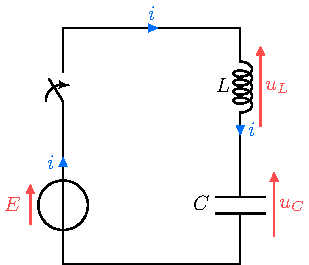
\includegraphics[width=.9\linewidth, draft=true]{lc_montant}
    }{%
      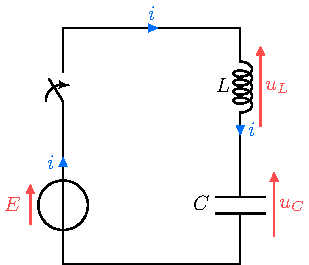
\includegraphics[width=.9\linewidth]{lc_montant}
    }%
    \captionof{figure}{}
  \end{center}
\end{tcb*}

\subsection{Équation différentielle et solution}
	\begin{tcb}[label=prop:eqdiffrc, sidebyside, righthand ratio=.4]
    (prop){Équation et solu$^\circ$ LC montant}
		L'équation différentielle $u_C(t)$ aux bornes d'un
		condensateur dans un circuit LC sous échelon montant est
			\[
		\psw{%
				\boxed{\dv[2]{u_C}{t} + \w_0{}^2u_C = \w_0{}^{2}E}
		}%
    \qav
		\psw{%
			\boxed{\w_0 = \frac{1}{\sqrt{LC}}}
		}%
			\]
		% avec \fbox{$\w_0 = \frac{1}{\sqrt{LC}}$} la pulsation propre.
		de conditions initiales
		%   (continuité de $u_C$ aux bornes de $C$
		% et de $i$ traversant $L$) sont
		\psw{%
			\begin{empheq}[box=\fbox]{gather*}
        u_C(0^-) = u_C(0^+) = 0
        \qet
        i(0^-) = i(0^+) = 0
			\end{empheq}
		}%
    \vspace{-15pt}
		\tcblower
    La solution de l'équation différentielle de la tension $u_C(t)$
    d'un circuit LC sous échelon montant avec $u_C(0) = 0$ et l'intensité en
    découlant sont
    \psw{%
      \begin{empheq}[box=\fbox]{align*}
        u_C(t) &= E(1 - \cos(\w_0t))\\
        i(t) &= CE\w_0\sin(\w_0t)
      \end{empheq}
    }%
	\end{tcb}

	\begin{tcb}[label=demo:eqdiffrc, sidebyside]
    (demo){Équation et solution LC montant}
    \tcbsubtitle{\fatbox{\textbf{Équation}}}
		Avec la loi des mailles,
		\psw{%
      \begin{DispWithArrows*}[fleqn, mathindent=5pt]
				u_L + u_C &= E
				\Arrow{$\DS u_L = L \dv{i}{t}$\\ et $\DS i = C \dv{u_C}{t}$}
				\\\Lra
				LC \dv[2]{u_C}{t} + u_C          &= E
				\Arrow{forme canonique}
				\\
				\Lra \dv[2]{u_C}{t} + \frac{1}{LC}u_C &= \frac{1}{LC}E
			\end{DispWithArrows*}
			% D'où le résultat. $L$ assure $i(0^+) = 0$ et $C$ assure $u_C(0^+) = 0$
			% par continuité.
		}%
  \tcbsubtitle{\fatbox{Solution}}
  Par changement de variable, on a
  \psw{%
    \[
      u_C(t) - E = A'\cos(\w_0 t + \f_0)
    \]
  }%
  \vspace{-15pt}
  \tcblower
  \begin{itemize}
    \item On trouve $\f_0$~:
          \psw{%
            \begin{gather*}
              i(0) = 0 = C \qty(\dv{u_C}{t})_0 = -A'\w_0 \sin(\f_0)
              \\\Lra
              \boxed{\f_0 = 0}
            \end{gather*}
          }%
          \vspace{-20pt}
    \item On trouve $A'$~:
          \psw{%
            \[
              u_C(0) - E = A' \cos(0)
              \Ra
              \boxed{A = -E}
            \]
          }%
          \vspace{-15pt}
  \end{itemize}
          \vspace{-15pt}
    \begin{gather*}
      \beforetext{Donc}
  \psw{%
      \boxed{u_C (t) = E \left( 1 - \cos(\w_0t) \right)}
  }%
    \end{gather*}
  On obtient ensuite $i$ avec la RCT~:
  \psw{%
    \[
      \boxed{i(t) = C \dv{u_c}{t} = CE \w_0 \sin(\w_0t)}
    \]
  }%
  \vspace{-15pt}
	\end{tcb}

% \subsection{Résolution de l'équation différentielle et graphique}
% \begin{tcb}[label=prop:ucsolu, sidebyside, righthand ratio=.3]
%   (prop){Solution LC montant}
%   La solution de l'équation différentielle de la tension $u_C(t)$
%   d'un circuit LC en charge avec $u_C(0) = 0$ et l'intensité en
%   découlant sont
%   \psw{%
%     \begin{empheq}[box=\fbox]{align*}
%       u_C(t) &= E(1 - \cos(\w_0t))\\
%       i(t)   &= CE\w_0\sin(\w_0t)
%     \end{empheq}
%   }%
%   \tcblower
%   \begin{center}
%     \sswitch{%
%       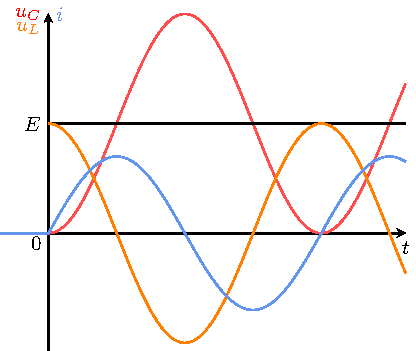
\includegraphics[width=\linewidth,
%         draft=true]{carac-lc_montant-harmonique}
%     }{%
%       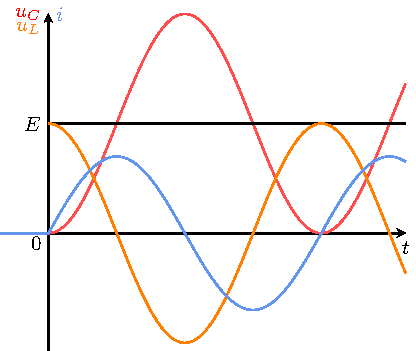
\includegraphics[width=\linewidth]{carac-lc_montant-harmonique}
%     }%
%     \captionof{figure}{}
%   \end{center}
% \end{tcb}
%
% \begin{tcb}[label=demo:rcsolu, sidebyside](demo)'r'{Solution LC montant}
%   D'après la propriété \ref{prop:chvar}, on sait que $u_C - E$ est
%   solution de l'équation homogène associée, donc on a
%   \psw{%
%     \[
%       u_C(t) - E = A'\cos(\w_0 t + \f_0)
%     \]
%   }%
%   \vspace{-15pt}
%   \begin{itemize}
%     \item On trouve $\f_0$~:
%           \psw{%
%             \begin{gather*}
%               i(0) = 0 = C \qty(\dv{u_C}{t})_0 = -A'\w_0 \sin(\f_0)
%               \quad \Ra
%               \boxed{\f_0 = 0}
%             \end{gather*}
%           }%
%           \vspace{-15pt}
%     \item On trouve $A'$~:
%           \psw{%
%             \[
%               u_C(0) - E = A' \cos(0)
%               \Ra
%               \boxed{A = -E}
%             \]
%           }%
%           \vspace{-15pt}
%   \end{itemize}
%   \tcblower
%   Donc
%   \psw{%
%     \[
%       \boxed{u_C (t) = E \left( 1 - \cos(\w_0t) \right)}
%     \]
%   }%
%   On obtient ensuite $i$ avec la relation courant-tension~:
%   \psw{%
%     \[
%       \boxed{i(t) = C \dv{u_c}{t} = CE \w_0 \sin(\w_0t)}
%     \]
%   }%
%   \vspace{-15pt}
% \end{tcb}

% \begin{tcbraster}[raster columns=2, raster equal height=rows, space to=\myspace]
% 	\begin{tcb}[label=rema:lccharge, ](rema){Valeur de $u_C$}
% 		On remarque aisément que $u_C$ atteint $2E$ par moment, ce qui pourrait
% 		paraître dérangeant puisqu'on donne une tension $E$ au système. En
% 		réalité ceci est tout à fait normal puisque $u_L = L\dv{i}{t}$ prend des
% 		valeurs négatives quand $i$ diminue~: la somme des deux fait bien $E$.
% 		\bigbreak
% 		On peut réaliser un bilan d'énergie pour vérifier que $\Ec_g =
% 			CE^2(1-\cos(\w_0t)) = \Ec_C + \Ec_L$, voir graphique ci-contre.
% 	\end{tcb}
% 	\begin{tcb}[add to natural height=\myspace](exem)'r'{Bilan d'énergie}
% 		\begin{center}
% 			\sswitch{%
% 				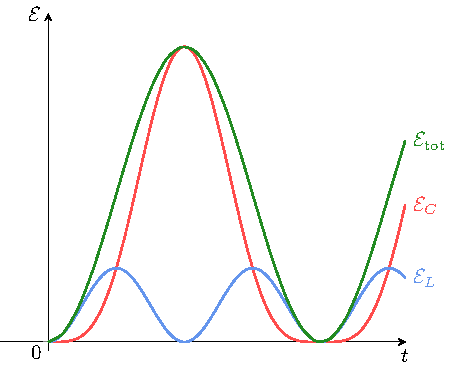
\includegraphics[width=\linewidth, draft=true]{carac-lc_montant-bilan}
% 			}{%
% 				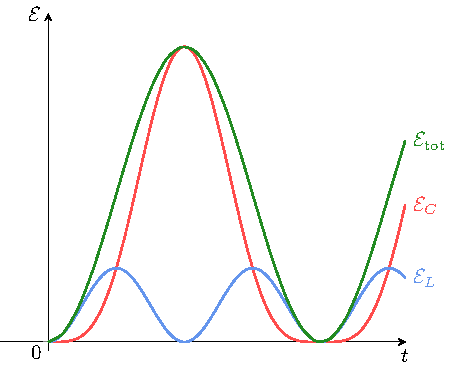
\includegraphics[width=\linewidth]{carac-lc_montant-bilan}
% 			}%
% 			\captionof{figure}{}
% 		\end{center}
% 	\end{tcb}
% \end{tcbraster}

% \subsection{Intérêt oscillateur harmonique}
%
% Le principal intérêt de l'observation régulière d'une oscillation est la mesure
% du temps. Une excitation quelconque (comme un échelon) produit un phénomène se
% reproduisant à intervalle régulier et fait alors apparaître un étalon temporel.
% Ce principe est utilisé~:
% \begin{itemize}
%   \item dans les \textbf{horloges mécaniques} à balancier~: on exploite le
%     mouvement régulier du pendule~;
%   \item dans les \textbf{horloges à ressort}~: la période est liée au rapport de
%         l'inertie et de la raideur du système~;
%   \item dans les \textbf{horloges électroniques}~: un cristal de quartz dont la
%     fréquence d'oscillation est précisément connue (en général une puissance de
%     2 en Hz)~;
%   \item dans les \textbf{horloges atomiques}~: on utilise la régularité des
%     oscillations des ondes électromagnétiques absorbées par un atome. L'actuelle
%     définition de la seconde est basée sur le fonctionnement d'une horloge
%     atomique.
% \end{itemize}

\vspace{-15pt}

\end{document}
